
% Default to the notebook output style

    


% Inherit from the specified cell style.




    
\documentclass[11pt]{article}

    
    
    \usepackage[T1]{fontenc}
    % Nicer default font (+ math font) than Computer Modern for most use cases
    \usepackage{mathpazo}

    % Basic figure setup, for now with no caption control since it's done
    % automatically by Pandoc (which extracts ![](path) syntax from Markdown).
    \usepackage{graphicx}
    % We will generate all images so they have a width \maxwidth. This means
    % that they will get their normal width if they fit onto the page, but
    % are scaled down if they would overflow the margins.
    \makeatletter
    \def\maxwidth{\ifdim\Gin@nat@width>\linewidth\linewidth
    \else\Gin@nat@width\fi}
    \makeatother
    \let\Oldincludegraphics\includegraphics
    % Set max figure width to be 80% of text width, for now hardcoded.
    \renewcommand{\includegraphics}[1]{\Oldincludegraphics[width=.8\maxwidth]{#1}}
    % Ensure that by default, figures have no caption (until we provide a
    % proper Figure object with a Caption API and a way to capture that
    % in the conversion process - todo).
    \usepackage{caption}
    \DeclareCaptionLabelFormat{nolabel}{}
    \captionsetup{labelformat=nolabel}

    \usepackage{adjustbox} % Used to constrain images to a maximum size 
    \usepackage{xcolor} % Allow colors to be defined
    \usepackage{enumerate} % Needed for markdown enumerations to work
    \usepackage{geometry} % Used to adjust the document margins
    \usepackage{amsmath} % Equations
    \usepackage{amssymb} % Equations
    \usepackage{textcomp} % defines textquotesingle
    % Hack from http://tex.stackexchange.com/a/47451/13684:
    \AtBeginDocument{%
        \def\PYZsq{\textquotesingle}% Upright quotes in Pygmentized code
    }
    \usepackage{upquote} % Upright quotes for verbatim code
    \usepackage{eurosym} % defines \euro
    \usepackage[mathletters]{ucs} % Extended unicode (utf-8) support
    \usepackage[utf8x]{inputenc} % Allow utf-8 characters in the tex document
    \usepackage{fancyvrb} % verbatim replacement that allows latex
    \usepackage{grffile} % extends the file name processing of package graphics 
                         % to support a larger range 
    % The hyperref package gives us a pdf with properly built
    % internal navigation ('pdf bookmarks' for the table of contents,
    % internal cross-reference links, web links for URLs, etc.)
    \usepackage{hyperref}
    \usepackage{longtable} % longtable support required by pandoc >1.10
    \usepackage{booktabs}  % table support for pandoc > 1.12.2
    \usepackage[inline]{enumitem} % IRkernel/repr support (it uses the enumerate* environment)
    \usepackage[normalem]{ulem} % ulem is needed to support strikethroughs (\sout)
                                % normalem makes italics be italics, not underlines
    

    
    
    % Colors for the hyperref package
    \definecolor{urlcolor}{rgb}{0,.145,.698}
    \definecolor{linkcolor}{rgb}{.71,0.21,0.01}
    \definecolor{citecolor}{rgb}{.12,.54,.11}

    % ANSI colors
    \definecolor{ansi-black}{HTML}{3E424D}
    \definecolor{ansi-black-intense}{HTML}{282C36}
    \definecolor{ansi-red}{HTML}{E75C58}
    \definecolor{ansi-red-intense}{HTML}{B22B31}
    \definecolor{ansi-green}{HTML}{00A250}
    \definecolor{ansi-green-intense}{HTML}{007427}
    \definecolor{ansi-yellow}{HTML}{DDB62B}
    \definecolor{ansi-yellow-intense}{HTML}{B27D12}
    \definecolor{ansi-blue}{HTML}{208FFB}
    \definecolor{ansi-blue-intense}{HTML}{0065CA}
    \definecolor{ansi-magenta}{HTML}{D160C4}
    \definecolor{ansi-magenta-intense}{HTML}{A03196}
    \definecolor{ansi-cyan}{HTML}{60C6C8}
    \definecolor{ansi-cyan-intense}{HTML}{258F8F}
    \definecolor{ansi-white}{HTML}{C5C1B4}
    \definecolor{ansi-white-intense}{HTML}{A1A6B2}

    % commands and environments needed by pandoc snippets
    % extracted from the output of `pandoc -s`
    \providecommand{\tightlist}{%
      \setlength{\itemsep}{0pt}\setlength{\parskip}{0pt}}
    \DefineVerbatimEnvironment{Highlighting}{Verbatim}{commandchars=\\\{\}}
    % Add ',fontsize=\small' for more characters per line
    \newenvironment{Shaded}{}{}
    \newcommand{\KeywordTok}[1]{\textcolor[rgb]{0.00,0.44,0.13}{\textbf{{#1}}}}
    \newcommand{\DataTypeTok}[1]{\textcolor[rgb]{0.56,0.13,0.00}{{#1}}}
    \newcommand{\DecValTok}[1]{\textcolor[rgb]{0.25,0.63,0.44}{{#1}}}
    \newcommand{\BaseNTok}[1]{\textcolor[rgb]{0.25,0.63,0.44}{{#1}}}
    \newcommand{\FloatTok}[1]{\textcolor[rgb]{0.25,0.63,0.44}{{#1}}}
    \newcommand{\CharTok}[1]{\textcolor[rgb]{0.25,0.44,0.63}{{#1}}}
    \newcommand{\StringTok}[1]{\textcolor[rgb]{0.25,0.44,0.63}{{#1}}}
    \newcommand{\CommentTok}[1]{\textcolor[rgb]{0.38,0.63,0.69}{\textit{{#1}}}}
    \newcommand{\OtherTok}[1]{\textcolor[rgb]{0.00,0.44,0.13}{{#1}}}
    \newcommand{\AlertTok}[1]{\textcolor[rgb]{1.00,0.00,0.00}{\textbf{{#1}}}}
    \newcommand{\FunctionTok}[1]{\textcolor[rgb]{0.02,0.16,0.49}{{#1}}}
    \newcommand{\RegionMarkerTok}[1]{{#1}}
    \newcommand{\ErrorTok}[1]{\textcolor[rgb]{1.00,0.00,0.00}{\textbf{{#1}}}}
    \newcommand{\NormalTok}[1]{{#1}}
    
    % Additional commands for more recent versions of Pandoc
    \newcommand{\ConstantTok}[1]{\textcolor[rgb]{0.53,0.00,0.00}{{#1}}}
    \newcommand{\SpecialCharTok}[1]{\textcolor[rgb]{0.25,0.44,0.63}{{#1}}}
    \newcommand{\VerbatimStringTok}[1]{\textcolor[rgb]{0.25,0.44,0.63}{{#1}}}
    \newcommand{\SpecialStringTok}[1]{\textcolor[rgb]{0.73,0.40,0.53}{{#1}}}
    \newcommand{\ImportTok}[1]{{#1}}
    \newcommand{\DocumentationTok}[1]{\textcolor[rgb]{0.73,0.13,0.13}{\textit{{#1}}}}
    \newcommand{\AnnotationTok}[1]{\textcolor[rgb]{0.38,0.63,0.69}{\textbf{\textit{{#1}}}}}
    \newcommand{\CommentVarTok}[1]{\textcolor[rgb]{0.38,0.63,0.69}{\textbf{\textit{{#1}}}}}
    \newcommand{\VariableTok}[1]{\textcolor[rgb]{0.10,0.09,0.49}{{#1}}}
    \newcommand{\ControlFlowTok}[1]{\textcolor[rgb]{0.00,0.44,0.13}{\textbf{{#1}}}}
    \newcommand{\OperatorTok}[1]{\textcolor[rgb]{0.40,0.40,0.40}{{#1}}}
    \newcommand{\BuiltInTok}[1]{{#1}}
    \newcommand{\ExtensionTok}[1]{{#1}}
    \newcommand{\PreprocessorTok}[1]{\textcolor[rgb]{0.74,0.48,0.00}{{#1}}}
    \newcommand{\AttributeTok}[1]{\textcolor[rgb]{0.49,0.56,0.16}{{#1}}}
    \newcommand{\InformationTok}[1]{\textcolor[rgb]{0.38,0.63,0.69}{\textbf{\textit{{#1}}}}}
    \newcommand{\WarningTok}[1]{\textcolor[rgb]{0.38,0.63,0.69}{\textbf{\textit{{#1}}}}}
    
    
    % Define a nice break command that doesn't care if a line doesn't already
    % exist.
    \def\br{\hspace*{\fill} \\* }
    % Math Jax compatability definitions
    \def\gt{>}
    \def\lt{<}
    % Document parameters
    \title{CE-157 Problem Set 3}
    
    
    

    % Pygments definitions
    
\makeatletter
\def\PY@reset{\let\PY@it=\relax \let\PY@bf=\relax%
    \let\PY@ul=\relax \let\PY@tc=\relax%
    \let\PY@bc=\relax \let\PY@ff=\relax}
\def\PY@tok#1{\csname PY@tok@#1\endcsname}
\def\PY@toks#1+{\ifx\relax#1\empty\else%
    \PY@tok{#1}\expandafter\PY@toks\fi}
\def\PY@do#1{\PY@bc{\PY@tc{\PY@ul{%
    \PY@it{\PY@bf{\PY@ff{#1}}}}}}}
\def\PY#1#2{\PY@reset\PY@toks#1+\relax+\PY@do{#2}}

\expandafter\def\csname PY@tok@gd\endcsname{\def\PY@tc##1{\textcolor[rgb]{0.63,0.00,0.00}{##1}}}
\expandafter\def\csname PY@tok@gu\endcsname{\let\PY@bf=\textbf\def\PY@tc##1{\textcolor[rgb]{0.50,0.00,0.50}{##1}}}
\expandafter\def\csname PY@tok@gt\endcsname{\def\PY@tc##1{\textcolor[rgb]{0.00,0.27,0.87}{##1}}}
\expandafter\def\csname PY@tok@gs\endcsname{\let\PY@bf=\textbf}
\expandafter\def\csname PY@tok@gr\endcsname{\def\PY@tc##1{\textcolor[rgb]{1.00,0.00,0.00}{##1}}}
\expandafter\def\csname PY@tok@cm\endcsname{\let\PY@it=\textit\def\PY@tc##1{\textcolor[rgb]{0.25,0.50,0.50}{##1}}}
\expandafter\def\csname PY@tok@vg\endcsname{\def\PY@tc##1{\textcolor[rgb]{0.10,0.09,0.49}{##1}}}
\expandafter\def\csname PY@tok@vi\endcsname{\def\PY@tc##1{\textcolor[rgb]{0.10,0.09,0.49}{##1}}}
\expandafter\def\csname PY@tok@vm\endcsname{\def\PY@tc##1{\textcolor[rgb]{0.10,0.09,0.49}{##1}}}
\expandafter\def\csname PY@tok@mh\endcsname{\def\PY@tc##1{\textcolor[rgb]{0.40,0.40,0.40}{##1}}}
\expandafter\def\csname PY@tok@cs\endcsname{\let\PY@it=\textit\def\PY@tc##1{\textcolor[rgb]{0.25,0.50,0.50}{##1}}}
\expandafter\def\csname PY@tok@ge\endcsname{\let\PY@it=\textit}
\expandafter\def\csname PY@tok@vc\endcsname{\def\PY@tc##1{\textcolor[rgb]{0.10,0.09,0.49}{##1}}}
\expandafter\def\csname PY@tok@il\endcsname{\def\PY@tc##1{\textcolor[rgb]{0.40,0.40,0.40}{##1}}}
\expandafter\def\csname PY@tok@go\endcsname{\def\PY@tc##1{\textcolor[rgb]{0.53,0.53,0.53}{##1}}}
\expandafter\def\csname PY@tok@cp\endcsname{\def\PY@tc##1{\textcolor[rgb]{0.74,0.48,0.00}{##1}}}
\expandafter\def\csname PY@tok@gi\endcsname{\def\PY@tc##1{\textcolor[rgb]{0.00,0.63,0.00}{##1}}}
\expandafter\def\csname PY@tok@gh\endcsname{\let\PY@bf=\textbf\def\PY@tc##1{\textcolor[rgb]{0.00,0.00,0.50}{##1}}}
\expandafter\def\csname PY@tok@ni\endcsname{\let\PY@bf=\textbf\def\PY@tc##1{\textcolor[rgb]{0.60,0.60,0.60}{##1}}}
\expandafter\def\csname PY@tok@nl\endcsname{\def\PY@tc##1{\textcolor[rgb]{0.63,0.63,0.00}{##1}}}
\expandafter\def\csname PY@tok@nn\endcsname{\let\PY@bf=\textbf\def\PY@tc##1{\textcolor[rgb]{0.00,0.00,1.00}{##1}}}
\expandafter\def\csname PY@tok@no\endcsname{\def\PY@tc##1{\textcolor[rgb]{0.53,0.00,0.00}{##1}}}
\expandafter\def\csname PY@tok@na\endcsname{\def\PY@tc##1{\textcolor[rgb]{0.49,0.56,0.16}{##1}}}
\expandafter\def\csname PY@tok@nb\endcsname{\def\PY@tc##1{\textcolor[rgb]{0.00,0.50,0.00}{##1}}}
\expandafter\def\csname PY@tok@nc\endcsname{\let\PY@bf=\textbf\def\PY@tc##1{\textcolor[rgb]{0.00,0.00,1.00}{##1}}}
\expandafter\def\csname PY@tok@nd\endcsname{\def\PY@tc##1{\textcolor[rgb]{0.67,0.13,1.00}{##1}}}
\expandafter\def\csname PY@tok@ne\endcsname{\let\PY@bf=\textbf\def\PY@tc##1{\textcolor[rgb]{0.82,0.25,0.23}{##1}}}
\expandafter\def\csname PY@tok@nf\endcsname{\def\PY@tc##1{\textcolor[rgb]{0.00,0.00,1.00}{##1}}}
\expandafter\def\csname PY@tok@si\endcsname{\let\PY@bf=\textbf\def\PY@tc##1{\textcolor[rgb]{0.73,0.40,0.53}{##1}}}
\expandafter\def\csname PY@tok@s2\endcsname{\def\PY@tc##1{\textcolor[rgb]{0.73,0.13,0.13}{##1}}}
\expandafter\def\csname PY@tok@nt\endcsname{\let\PY@bf=\textbf\def\PY@tc##1{\textcolor[rgb]{0.00,0.50,0.00}{##1}}}
\expandafter\def\csname PY@tok@nv\endcsname{\def\PY@tc##1{\textcolor[rgb]{0.10,0.09,0.49}{##1}}}
\expandafter\def\csname PY@tok@s1\endcsname{\def\PY@tc##1{\textcolor[rgb]{0.73,0.13,0.13}{##1}}}
\expandafter\def\csname PY@tok@dl\endcsname{\def\PY@tc##1{\textcolor[rgb]{0.73,0.13,0.13}{##1}}}
\expandafter\def\csname PY@tok@ch\endcsname{\let\PY@it=\textit\def\PY@tc##1{\textcolor[rgb]{0.25,0.50,0.50}{##1}}}
\expandafter\def\csname PY@tok@m\endcsname{\def\PY@tc##1{\textcolor[rgb]{0.40,0.40,0.40}{##1}}}
\expandafter\def\csname PY@tok@gp\endcsname{\let\PY@bf=\textbf\def\PY@tc##1{\textcolor[rgb]{0.00,0.00,0.50}{##1}}}
\expandafter\def\csname PY@tok@sh\endcsname{\def\PY@tc##1{\textcolor[rgb]{0.73,0.13,0.13}{##1}}}
\expandafter\def\csname PY@tok@ow\endcsname{\let\PY@bf=\textbf\def\PY@tc##1{\textcolor[rgb]{0.67,0.13,1.00}{##1}}}
\expandafter\def\csname PY@tok@sx\endcsname{\def\PY@tc##1{\textcolor[rgb]{0.00,0.50,0.00}{##1}}}
\expandafter\def\csname PY@tok@bp\endcsname{\def\PY@tc##1{\textcolor[rgb]{0.00,0.50,0.00}{##1}}}
\expandafter\def\csname PY@tok@c1\endcsname{\let\PY@it=\textit\def\PY@tc##1{\textcolor[rgb]{0.25,0.50,0.50}{##1}}}
\expandafter\def\csname PY@tok@fm\endcsname{\def\PY@tc##1{\textcolor[rgb]{0.00,0.00,1.00}{##1}}}
\expandafter\def\csname PY@tok@o\endcsname{\def\PY@tc##1{\textcolor[rgb]{0.40,0.40,0.40}{##1}}}
\expandafter\def\csname PY@tok@kc\endcsname{\let\PY@bf=\textbf\def\PY@tc##1{\textcolor[rgb]{0.00,0.50,0.00}{##1}}}
\expandafter\def\csname PY@tok@c\endcsname{\let\PY@it=\textit\def\PY@tc##1{\textcolor[rgb]{0.25,0.50,0.50}{##1}}}
\expandafter\def\csname PY@tok@mf\endcsname{\def\PY@tc##1{\textcolor[rgb]{0.40,0.40,0.40}{##1}}}
\expandafter\def\csname PY@tok@err\endcsname{\def\PY@bc##1{\setlength{\fboxsep}{0pt}\fcolorbox[rgb]{1.00,0.00,0.00}{1,1,1}{\strut ##1}}}
\expandafter\def\csname PY@tok@mb\endcsname{\def\PY@tc##1{\textcolor[rgb]{0.40,0.40,0.40}{##1}}}
\expandafter\def\csname PY@tok@ss\endcsname{\def\PY@tc##1{\textcolor[rgb]{0.10,0.09,0.49}{##1}}}
\expandafter\def\csname PY@tok@sr\endcsname{\def\PY@tc##1{\textcolor[rgb]{0.73,0.40,0.53}{##1}}}
\expandafter\def\csname PY@tok@mo\endcsname{\def\PY@tc##1{\textcolor[rgb]{0.40,0.40,0.40}{##1}}}
\expandafter\def\csname PY@tok@kd\endcsname{\let\PY@bf=\textbf\def\PY@tc##1{\textcolor[rgb]{0.00,0.50,0.00}{##1}}}
\expandafter\def\csname PY@tok@mi\endcsname{\def\PY@tc##1{\textcolor[rgb]{0.40,0.40,0.40}{##1}}}
\expandafter\def\csname PY@tok@kn\endcsname{\let\PY@bf=\textbf\def\PY@tc##1{\textcolor[rgb]{0.00,0.50,0.00}{##1}}}
\expandafter\def\csname PY@tok@cpf\endcsname{\let\PY@it=\textit\def\PY@tc##1{\textcolor[rgb]{0.25,0.50,0.50}{##1}}}
\expandafter\def\csname PY@tok@kr\endcsname{\let\PY@bf=\textbf\def\PY@tc##1{\textcolor[rgb]{0.00,0.50,0.00}{##1}}}
\expandafter\def\csname PY@tok@s\endcsname{\def\PY@tc##1{\textcolor[rgb]{0.73,0.13,0.13}{##1}}}
\expandafter\def\csname PY@tok@kp\endcsname{\def\PY@tc##1{\textcolor[rgb]{0.00,0.50,0.00}{##1}}}
\expandafter\def\csname PY@tok@w\endcsname{\def\PY@tc##1{\textcolor[rgb]{0.73,0.73,0.73}{##1}}}
\expandafter\def\csname PY@tok@kt\endcsname{\def\PY@tc##1{\textcolor[rgb]{0.69,0.00,0.25}{##1}}}
\expandafter\def\csname PY@tok@sc\endcsname{\def\PY@tc##1{\textcolor[rgb]{0.73,0.13,0.13}{##1}}}
\expandafter\def\csname PY@tok@sb\endcsname{\def\PY@tc##1{\textcolor[rgb]{0.73,0.13,0.13}{##1}}}
\expandafter\def\csname PY@tok@sa\endcsname{\def\PY@tc##1{\textcolor[rgb]{0.73,0.13,0.13}{##1}}}
\expandafter\def\csname PY@tok@k\endcsname{\let\PY@bf=\textbf\def\PY@tc##1{\textcolor[rgb]{0.00,0.50,0.00}{##1}}}
\expandafter\def\csname PY@tok@se\endcsname{\let\PY@bf=\textbf\def\PY@tc##1{\textcolor[rgb]{0.73,0.40,0.13}{##1}}}
\expandafter\def\csname PY@tok@sd\endcsname{\let\PY@it=\textit\def\PY@tc##1{\textcolor[rgb]{0.73,0.13,0.13}{##1}}}

\def\PYZbs{\char`\\}
\def\PYZus{\char`\_}
\def\PYZob{\char`\{}
\def\PYZcb{\char`\}}
\def\PYZca{\char`\^}
\def\PYZam{\char`\&}
\def\PYZlt{\char`\<}
\def\PYZgt{\char`\>}
\def\PYZsh{\char`\#}
\def\PYZpc{\char`\%}
\def\PYZdl{\char`\$}
\def\PYZhy{\char`\-}
\def\PYZsq{\char`\'}
\def\PYZdq{\char`\"}
\def\PYZti{\char`\~}
% for compatibility with earlier versions
\def\PYZat{@}
\def\PYZlb{[}
\def\PYZrb{]}
\makeatother


    % Exact colors from NB
    \definecolor{incolor}{rgb}{0.0, 0.0, 0.5}
    \definecolor{outcolor}{rgb}{0.545, 0.0, 0.0}



    
    % Prevent overflowing lines due to hard-to-break entities
    \sloppy 
    % Setup hyperref package
    \hypersetup{
      breaklinks=true,  % so long urls are correctly broken across lines
      colorlinks=true,
      urlcolor=urlcolor,
      linkcolor=linkcolor,
      citecolor=citecolor,
      }
    % Slightly bigger margins than the latex defaults
    
    \geometry{verbose,tmargin=1in,bmargin=1in,lmargin=1in,rmargin=1in}
    
    

    \begin{document}
    
    
    \maketitle
    
    

    
    \section{CE-157 Problem Set 3}\label{ce-157-problem-set-3}

Run the cell below and continue onwards! It is just needed to run the
initial code needed to run the rest of the functions in this problem
set.

    \begin{Verbatim}[commandchars=\\\{\}]
{\color{incolor}In [{\color{incolor}2}]:} \PY{k+kn}{import} \PY{n+nn}{matplotlib}
        \PY{n}{matplotlib}\PY{o}{.}\PY{n}{use}\PY{p}{(}\PY{l+s+s1}{\PYZsq{}}\PY{l+s+s1}{Agg}\PY{l+s+s1}{\PYZsq{}}\PY{p}{)}
        \PY{o}{\PYZpc{}}\PY{k}{matplotlib} inline
        \PY{k+kn}{import} \PY{n+nn}{matplotlib.pyplot} \PY{k+kn}{as} \PY{n+nn}{plt}
        \PY{k+kn}{from} \PY{n+nn}{datascience} \PY{k+kn}{import} \PY{o}{*}
        \PY{k+kn}{import} \PY{n+nn}{numpy} \PY{k+kn}{as} \PY{n+nn}{np}
        \PY{k+kn}{import} \PY{n+nn}{pandas} \PY{k+kn}{as} \PY{n+nn}{pd}
\end{Verbatim}


    \paragraph{Shortcuts for column names}\label{shortcuts-for-column-names}

    \begin{longtable}[]{@{}ll@{}}
\toprule
\begin{minipage}[b]{0.20\columnwidth}\raggedright\strut
Column Name\strut
\end{minipage} & \begin{minipage}[b]{0.13\columnwidth}\raggedright\strut
Description\strut
\end{minipage}\tabularnewline
\midrule
\endhead
\begin{minipage}[t]{0.20\columnwidth}\raggedright\strut
co2\_commulative\strut
\end{minipage} & \begin{minipage}[t]{0.13\columnwidth}\raggedright\strut
Historical Emissions A Cumulative CO2 emission from energy, 1850-2007
(million tonnes)\strut
\end{minipage}\tabularnewline
\begin{minipage}[t]{0.20\columnwidth}\raggedright\strut
ghg\_commulative\strut
\end{minipage} & \begin{minipage}[t]{0.13\columnwidth}\raggedright\strut
Historical Emissions B Cumulative GHG Emissions, 1990-2010 (million
tonnes CO2 equivalent)\strut
\end{minipage}\tabularnewline
\begin{minipage}[t]{0.20\columnwidth}\raggedright\strut
ghg\_2010\strut
\end{minipage} & \begin{minipage}[t]{0.13\columnwidth}\raggedright\strut
Current GHG Emissions Total GHG Emissions, 2010 (million tonnes CO2
equivalent)\strut
\end{minipage}\tabularnewline
\begin{minipage}[t]{0.20\columnwidth}\raggedright\strut
co2\_2011\strut
\end{minipage} & \begin{minipage}[t]{0.13\columnwidth}\raggedright\strut
Current CO2 Emissions CO2 emissions from fossil fuel combustion, 2011
(million tonnes)\strut
\end{minipage}\tabularnewline
\begin{minipage}[t]{0.20\columnwidth}\raggedright\strut
change\_1971\_2011\strut
\end{minipage} & \begin{minipage}[t]{0.13\columnwidth}\raggedright\strut
Change from 1971--2011 (\%)\strut
\end{minipage}\tabularnewline
\begin{minipage}[t]{0.20\columnwidth}\raggedright\strut
change\_1990\_2011\strut
\end{minipage} & \begin{minipage}[t]{0.13\columnwidth}\raggedright\strut
Change from 1990--2011 (\%)\strut
\end{minipage}\tabularnewline
\begin{minipage}[t]{0.20\columnwidth}\raggedright\strut
total\_footprint\strut
\end{minipage} & \begin{minipage}[t]{0.13\columnwidth}\raggedright\strut
Total carbon footprint Footprint of all goods and services consumed
(million tonnes CO2 equivalent)\strut
\end{minipage}\tabularnewline
\begin{minipage}[t]{0.20\columnwidth}\raggedright\strut
pop\_2010\strut
\end{minipage} & \begin{minipage}[t]{0.13\columnwidth}\raggedright\strut
Population 2010\strut
\end{minipage}\tabularnewline
\begin{minipage}[t]{0.20\columnwidth}\raggedright\strut
gdp\_ppp\_2010\strut
\end{minipage} & \begin{minipage}[t]{0.13\columnwidth}\raggedright\strut
GDP-PPP 2010 (Million \$ (2005))\strut
\end{minipage}\tabularnewline
\begin{minipage}[t]{0.20\columnwidth}\raggedright\strut
hdi\_2011\strut
\end{minipage} & \begin{minipage}[t]{0.13\columnwidth}\raggedright\strut
HDI, 2011\strut
\end{minipage}\tabularnewline
\begin{minipage}[t]{0.20\columnwidth}\raggedright\strut
hdi\_change\_1990\_2011\strut
\end{minipage} & \begin{minipage}[t]{0.13\columnwidth}\raggedright\strut
HDI Change from 1990-2011 (\%)\strut
\end{minipage}\tabularnewline
\begin{minipage}[t]{0.20\columnwidth}\raggedright\strut
gender\_inequality\_2012\strut
\end{minipage} & \begin{minipage}[t]{0.13\columnwidth}\raggedright\strut
Gender Inequality Index Value, 2012\strut
\end{minipage}\tabularnewline
\begin{minipage}[t]{0.20\columnwidth}\raggedright\strut
maternal\_2010\strut
\end{minipage} & \begin{minipage}[t]{0.13\columnwidth}\raggedright\strut
Maternal Mortality Ratio, 2010\strut
\end{minipage}\tabularnewline
\bottomrule
\end{longtable}

    \paragraph{GENERAL NOTES:}\label{general-notes}

\begin{enumerate}
\def\labelenumi{\arabic{enumi}.}
\tightlist
\item
  \textbf{A tip to navigate Jupyter}: Pull up the documentation for any
  function in Jupyter by typing the function name, then
  \texttt{\textless{}Shift\textgreater{}-\textless{}Tab\textgreater{}}
  on your keyboard. This is very useful when you want to know what
  arguments a function takes, or the order of the arguments in a
  function. You can press\texttt{\textless{}Tab\textgreater{}} multiple
  times to expand the docs.
\item
  \textbf{How to write comments in python?}

  \begin{itemize}
  \tightlist
  \item
    Type 1: You can create a single-line comment by simply beginning a
    line with a hash (\#). These are usually for yourself. Look at the
    example below for reference.
  \item
    Type 2: You can use multi-line comments or paragraphs that serve as
    documentation for others reading your code. Look at the example
    below for reference.
  \item
    Throughout the notebook, you will find several comments made for you
    so that you can understand what the code does. We will also ask you
    to comment some lines of codes to make sure you don't get any
    assertion errors.
  \end{itemize}
\end{enumerate}

source: https://www.pythonforbeginners.com/comments/comments-in-python

    \begin{Verbatim}[commandchars=\\\{\}]
{\color{incolor}In [{\color{incolor}3}]:} \PY{c+c1}{\PYZsh{} Type 1:}
        \PY{c+c1}{\PYZsh{}This would be a comment in Python}
        
        \PY{c+c1}{\PYZsh{} Type 2:}
        \PY{k}{def} \PY{n+nf}{comment}\PY{p}{(}\PY{n}{x}\PY{p}{)}\PY{p}{:}
            \PY{l+s+sd}{\PYZdq{}\PYZdq{}\PYZdq{}}
        \PY{l+s+sd}{    This function prints the comments stored in the varaible x.}
        
        \PY{l+s+sd}{    Arguments:}
        \PY{l+s+sd}{    x: string }
        \PY{l+s+sd}{    }
        \PY{l+s+sd}{    Example: }
        \PY{l+s+sd}{    \PYZgt{} x = \PYZdq{}Hello world!\PYZdq{}}
        \PY{l+s+sd}{    \PYZgt{} comment(x) }
        \PY{l+s+sd}{    \PYZgt{}\PYZgt{}\PYZgt{} This function prints the comment stored the  in varible x. The comment is: Hello World!}
        \PY{l+s+sd}{    }
        \PY{l+s+sd}{    \PYZdq{}\PYZdq{}\PYZdq{}}
            \PY{k}{print}\PY{p}{(}\PY{n}{f}\PY{l+s+s2}{\PYZdq{}}\PY{l+s+s2}{This function prints the comment stored the  in varible x. The comment is: \PYZob{}x\PYZcb{}}\PY{l+s+s2}{\PYZdq{}}\PY{p}{)}
\end{Verbatim}


    \paragraph{Alright! Let's begin!}\label{alright-lets-begin}

In this problem set, you will dive into some publicly available data on
climate change, economic growth, and human development in an attempt to
understand a little about the complex relationships between these
parameters. With each chart you create, be sure to label your axes,
create a chart title, and provide a simple regression line (including
the R2 value). Note that you don't need a chart legend if you only have
one set of data. Remember -- presentation is important! Also remember
that a robust analysis would use far more in depth statistics, in
particular focusing on each component of your regression model, both the
size of the effect of each component as well as the significance, but
for the purposes of this problem set linear regression slopes and R2
values will do.

    

    \subsection{Table of Contents}\label{table-of-contents}

1 - Section \ref{section1}

2 - Section \ref{section2}

3 - Section \ref{section3}

4 - Section \ref{section4}

5 - Section \ref{section5}

6 - Section \ref{section6}

7 - Section \ref{section7}

    

    The data is in a table named \texttt{problem\_set} (Run the next cell to
see what it looks like).

    \begin{Verbatim}[commandchars=\\\{\}]
{\color{incolor}In [{\color{incolor}4}]:} \PY{n}{problem\PYZus{}set}\PY{o}{=}\PY{n}{Table}\PY{o}{.}\PY{n}{read\PYZus{}table}\PY{p}{(}\PY{l+s+s1}{\PYZsq{}}\PY{l+s+s1}{problem\PYZus{}set.csv}\PY{l+s+s1}{\PYZsq{}}\PY{p}{)}
        \PY{n}{problem\PYZus{}set}
\end{Verbatim}


\begin{Verbatim}[commandchars=\\\{\}]
{\color{outcolor}Out[{\color{outcolor}4}]:} countries         | co2\_cummulative | ghg\_cummulative | ghg\_2010 | co2\_2011 | change\_1971\_2011 | change\_1990\_2011 | total\_footprint | pop\_2010   | gdp\_ppp\_2010 | hdi\_2011 | hdi\_change\_1990\_2011 | gender\_inequality\_2012 | maternal\_2010
        Afghanistan       | 72.4            | 349.34          | 24.94    | nan      | nan              | nan              | nan             | 28,397,812 | 33596        | 0.371    | 50.81                | 0.712                  | 460
        Albania           | 227.9           | 143.81          | 6.57     |   3.9    | -0.3             | -38              | 5.4             | 3,150,143  | 24545        | 0.748    | 13.16                | 0.251                  | 27
        Algeria           | 2,272.40        | 2618.81         | 169.42   |   103.9  | 1064.8           | 97               | nan             | 37,062,820 | 269075       | 0.711    | 26.51                | 0.391                  | 97
        Angola            | 305.3           | 3300.97         | 219.84   |   15.7   | 845.5            | 292              | nan             | 19,549,124 | 98686        | 0.504    | nan                  | nan                    | 450
        Antigua \& Barbuda | 16.6            | 14.17           | 1.2      | nan      | nan              | nan              | nan             | 87,233     | 1541         | 0.759    | nan                  | nan                    | nan
        Argentina         | 5,894.80        | 6308.23         | 359.01   |   183.6  | 121.8            | 83.8             | 165.5           | 40,374,224 | 580427       | 0.81     | 15.55                | 0.38                   | 77
        Armenia           | 505.6           | 183.45          | 13.43    |   4.7    | nan              | -77.2            | 6               | 2,963,496  | 15153        | 0.726    | 15.61                | 0.34                   | 30
        Australia         | 13,108.50       | 10252.5         | 587.53   |   396.8  | 175.3            | 52.6             | 297             | 22,065,300 | 763921       | 0.936    | 6.36                 | 0.115                  | 7
        Austria           | 4,541.90        | 1712.92         | 84.28    |   68.5   | 40.6             | 21.4             | 99.8            | 8,389,771  | 296268       | 0.894    | 12.17                | 0.102                  | 4
        Azerbaijan        | 2,323.70        | 1218.83         | 64.21    |   26.8   | nan              | -51.3            | 30.3            | 9,054,332  | 80696        | 0.732    | nan                  | 0.323                  | 43
        {\ldots} (176 rows omitted)
\end{Verbatim}
            
    \subsection{Introduction to Ploting }\label{introduction-to-ploting}

\paragraph{A quick tutorial on how to plot with Numpy and
Matplotlib}\label{a-quick-tutorial-on-how-to-plot-with-numpy-and-matplotlib}

Ploting is one of the most important steps of exploratory data analysis.
It can help us uncover things we could not perceive by simply looking at
summary statistics or at the first 10 rows of our data set. Python has
to very helpful libraries that contain many handy functions to make
plotting easy and intuitive namely Numpy and Matplotlib.

Some of the functions we might find useful in this problem set are: -
Plot - Scatter

    \paragraph{Scatter Plots}\label{scatter-plots}

Lets explore the \textbf{scattter} function. Using scattter plot you're
able to take any two columns of a table, and plot them quite easily! For
example, the scatter plot for Total GHG Emissions, 2010 vs. GDP-PPP 2010
(Million \$ (2005)) should look like:

    Now, lets crete a function that will help us with create a scatter plot.

    \begin{Verbatim}[commandchars=\\\{\}]
{\color{incolor}In [{\color{incolor}5}]:} \PY{k}{def} \PY{n+nf}{scatter}\PY{p}{(}\PY{n}{x}\PY{p}{,} \PY{n}{y}\PY{p}{)}\PY{p}{:}
            \PY{l+s+sd}{\PYZdq{}\PYZdq{}\PYZdq{}}
        \PY{l+s+sd}{    Generate a scatter plot using x and y}
        
        \PY{l+s+sd}{    Arguments:}
        \PY{l+s+sd}{    x \PYZhy{}\PYZhy{} the vector of values x}
        \PY{l+s+sd}{    y \PYZhy{}\PYZhy{} the vector of values y}
        \PY{l+s+sd}{    }
        \PY{l+s+sd}{    Example:}
        \PY{l+s+sd}{    x = problem\PYZus{}set.column(\PYZdq{}column name\PYZdq{})}
        \PY{l+s+sd}{    y = problem\PYZus{}set.column(\PYZdq{}column name\PYZdq{})}
        \PY{l+s+sd}{    p1= scatter(x,y)}
        \PY{l+s+sd}{    }
        \PY{l+s+sd}{    Tip: You can plt.scatter(x,y, s=6) to change the size of your points to 6. Try any number! }
        \PY{l+s+sd}{    \PYZdq{}\PYZdq{}\PYZdq{}}
            \PY{n}{plt}\PY{o}{.}\PY{n}{figure}\PY{p}{(}\PY{n}{figsize}\PY{o}{=}\PY{p}{(}\PY{l+m+mi}{8}\PY{p}{,} \PY{l+m+mi}{6}\PY{p}{)}\PY{p}{)}
            \PY{n}{plt}\PY{o}{.}\PY{n}{scatter}\PY{p}{(}\PY{n}{x}\PY{p}{,}\PY{n}{y}\PY{p}{)}  
            
        
        \PY{c+c1}{\PYZsh{} Do not worry too much about the implementation yet, we will discuss the details later.}
\end{Verbatim}


    \paragraph{NOTE: Make sure to save your plots to a variable as it is
done in the example (e.g. p1=scatter(x,y)). You will need this to run
future
functions.}\label{note-make-sure-to-save-your-plots-to-a-variable-as-it-is-done-in-the-example-e.g.-p1scatterxy.-you-will-need-this-to-run-future-functions.}

    \paragraph{YOUR TURN}\label{your-turn}

\begin{enumerate}
\def\labelenumi{\arabic{enumi}.}
\tightlist
\item
  Complete the following function by filling in the (...) below with the
  appropiate arguments.
\item
  Use {[}plot, xlab, ylab, plot\_title{]} to fill in the blanks. Note
  not all of them are going to be used.
\end{enumerate}

Make sure to comment out the line that reads \textbf{"raise
NotImplementedError()"} by using \textbf{\#} once you have completed the
question.

    \begin{Verbatim}[commandchars=\\\{\}]
{\color{incolor}In [{\color{incolor}6}]:}  \PY{k}{def} \PY{n+nf}{put\PYZus{}label\PYZus{}on\PYZus{}plot}\PY{p}{(}\PY{n}{plot}\PY{p}{,} \PY{n}{xlab}\PY{p}{,} \PY{n}{ylab}\PY{p}{,} \PY{n}{plot\PYZus{}title}\PY{p}{)}\PY{p}{:}
            \PY{l+s+sd}{\PYZdq{}\PYZdq{}\PYZdq{}}
        \PY{l+s+sd}{    Generate labels for a plot using plot, xlab, ylab, and plot title}
        
        \PY{l+s+sd}{    Arguments:}
        \PY{l+s+sd}{    plot \PYZhy{}\PYZhy{} Any plot. For instance, a plot created using the scatter function above}
        \PY{l+s+sd}{    xlab \PYZhy{}\PYZhy{} Label for x\PYZhy{}axis }
        \PY{l+s+sd}{    ylab \PYZhy{}\PYZhy{} Label for y\PYZhy{}axis }
        \PY{l+s+sd}{    plot\PYZus{}title \PYZhy{}\PYZhy{} Title for your plot }
        \PY{l+s+sd}{    }
        \PY{l+s+sd}{       }
        \PY{l+s+sd}{    Example:}
        \PY{l+s+sd}{    x = problem\PYZus{}set.column(\PYZdq{}column name\PYZdq{})}
        \PY{l+s+sd}{    y = problem\PYZus{}set.column(\PYZdq{}column name\PYZdq{})}
        \PY{l+s+sd}{    my\PYZus{}scatter = scatter(x, y)}
        \PY{l+s+sd}{    put\PYZus{}label\PYZus{}on\PYZus{}plot(my\PYZus{}scatter, \PYZdq{}name for x axis\PYZdq{}, \PYZdq{}name for y axis \PYZdq{}, \PYZdq{}plot title\PYZdq{})}
        \PY{l+s+sd}{    \PYZdq{}\PYZdq{}\PYZdq{}}
            
            \PY{n}{plt}\PY{o}{.}\PY{n}{xlabel}\PY{p}{(}\PY{o}{.}\PY{o}{.}\PY{o}{.}\PY{p}{)}  \PY{c+c1}{\PYZsh{} YOUR CODE HERE}
            \PY{n}{plt}\PY{o}{.}\PY{n}{ylabel}\PY{p}{(}\PY{o}{.}\PY{o}{.}\PY{o}{.}\PY{p}{)}  \PY{c+c1}{\PYZsh{} YOUR CODE HERE}
            \PY{n}{plt}\PY{o}{.}\PY{n}{title}\PY{p}{(}\PY{o}{.}\PY{o}{.}\PY{o}{.}\PY{p}{)}   \PY{c+c1}{\PYZsh{} YOUR CODE HERE}
            
        \PY{k}{raise} \PY{n+ne}{NotImplementedError}\PY{p}{(}\PY{p}{)}
\end{Verbatim}


    \begin{Verbatim}[commandchars=\\\{\}]

        ---------------------------------------------------------------------------

        NotImplementedError                       Traceback (most recent call last)

        <ipython-input-6-74ee5503ca23> in <module>
         21    plt.title({\ldots})   \# YOUR CODE HERE
         22 
    ---> 23 raise NotImplementedError()
    

        NotImplementedError: 

    \end{Verbatim}

    \paragraph{Labeling:}\label{labeling}

If we look back the scattter plot created above we will notice that it
is very hard to interpret the plot since we do not know what x and y
mean. For us to make any inferences or useful obervations on the plot we
need more context. The following functions are very useful to help you,
and others reading your plots understand what you are talking about.
Some helpful functions that we can use to enhance out plots are:

\begin{itemize}
\tightlist
\item
  plt.xlabel()
\item
  plt.ylabel()
\item
  plt.title()
\end{itemize}

    Now we will write a utility function that will allow us to label our
plots.

    \paragraph{\texorpdfstring{Running the two functions above on
\textbf{Total GHG Emissions, 2010} and \textbf{GDP-PPP 2010 (Million
(2005))} should produce the following
plot:}{Running the two functions above on Total GHG Emissions, 2010 and GDP-PPP 2010 (Million (2005)) should produce the following plot:}}\label{running-the-two-functions-above-on-total-ghg-emissions-2010-and-gdp-ppp-2010-million-2005-should-produce-the-following-plot}

    

    \paragraph{YOUR TURN }\label{your-turn}

\begin{itemize}
\tightlist
\item
  Use the functions above (scatter and put\_label\_on\_plot) to rereate
  the plot above.
\item
  Make sure to replace the ... with your solution
\item
  Do not forget to give your plot meaningful labels.
\item
  Do not forget to comment out the implementation test.
\end{itemize}

Tips: * How do I know if my labels are good enough? * Can someone who is
not taking the class understand the your plot without any additional
infromation? If yes, you did it! If not, try to find more meaningful
names for your plot and labels.

    \begin{Verbatim}[commandchars=\\\{\}]
{\color{incolor}In [{\color{incolor} }]:} \PY{c+c1}{\PYZsh{} YOUR CODE HERE}
        \PY{n}{x} \PY{o}{=}  \PY{n}{problem\PYZus{}set}\PY{o}{.}\PY{n}{column}\PY{p}{(}\PY{l+s+s2}{\PYZdq{}}\PY{l+s+s2}{ghg\PYZus{}2010}\PY{l+s+s2}{\PYZdq{}}\PY{p}{)}
        \PY{n}{y} \PY{o}{=} \PY{n}{problem\PYZus{}set}\PY{o}{.}\PY{n}{column}\PY{p}{(}\PY{l+s+s2}{\PYZdq{}}\PY{l+s+s2}{gdp\PYZus{}ppp\PYZus{}2010}\PY{l+s+s2}{\PYZdq{}}\PY{p}{)}
        
        \PY{n}{test\PYZus{}plot} \PY{o}{=} \PY{n}{scatter}\PY{p}{(}\PY{o}{.}\PY{o}{.}\PY{o}{.}\PY{p}{,}\PY{o}{.}\PY{o}{.}\PY{p}{)}
        
        \PY{n}{put\PYZus{}label\PYZus{}on\PYZus{}plot}\PY{p}{(}\PY{n}{test\PYZus{}plot}\PY{p}{,} \PY{o}{.}\PY{o}{.}\PY{o}{.}\PY{p}{,} \PY{o}{.}\PY{o}{.}\PY{o}{.}\PY{p}{,} \PY{o}{.}\PY{o}{.}\PY{o}{.}\PY{p}{)} 
        
        
        \PY{k}{raise} \PY{n+ne}{NotImplementedError}\PY{p}{(}\PY{p}{)}
\end{Verbatim}


    \subsection{Correlation }\label{correlation}

    \paragraph{\texorpdfstring{The correlation coefficient -
\emph{r}}{The correlation coefficient - r}}\label{the-correlation-coefficient---r}

\begin{itemize}
\tightlist
\item
  r is a numerical measure of correlation ranging from -1 to 1. It gives
  us information about the strength of the relationship between two
  variables.
\item
  Although there are different types of correlation, we will use
  "Pearson's correlation" or "Pearson's R".
\end{itemize}

\paragraph{\texorpdfstring{How to interpret \emph{r}
?}{How to interpret r ?}}\label{how-to-interpret-r}

\begin{itemize}
\tightlist
\item
  r=1: For every unit increase in a variable, say X, there is a positive
  increase of a fixed proportion on the other varaible, say Y.
\item
  r=-1: For every unit increase in a Variable, say X, the is a negative
  increase of a fixed proportion on the other varaible, say Y.
\item
  r=0: For every unit increase in a variable, say X, there is not a
  negative or positive increase on the other variable, say Y. This means
  that the two variables are un-correlated.
\end{itemize}

    \paragraph{These are some examples of different correlatiosn
r}\label{these-are-some-examples-of-different-correlatiosn-r}

    source: mathsisfun.com

    Now that you have a visual and conceptual idea of what correlation is,
we can use the functions defined below to calculate the corralation for
the variables in your data set.

You do not have to worry about understanding the implementation of the
two functions below, you just need to know how to use and interpret the
results for the \emph{correlation} function we created for you.

If you would like to learn more about how to obtain the corraltion
coefficient please visit
https://www.inferentialthinking.com/chapters/15/1/Correlation for more
details.

    \begin{Verbatim}[commandchars=\\\{\}]
{\color{incolor}In [{\color{incolor} }]:} \PY{k}{def} \PY{n+nf}{standard\PYZus{}units}\PY{p}{(}\PY{n}{x}\PY{p}{)}\PY{p}{:}
            \PY{l+s+sd}{\PYZdq{}\PYZdq{}\PYZdq{}}
        \PY{l+s+sd}{    Convert any array of numbers to standard units.}
        \PY{l+s+sd}{    \PYZdq{}\PYZdq{}\PYZdq{}}
            
            \PY{k}{return} \PY{p}{(}\PY{n}{x} \PY{o}{\PYZhy{}} \PY{n}{np}\PY{o}{.}\PY{n}{average}\PY{p}{(}\PY{n}{x}\PY{p}{)}\PY{p}{)}\PY{o}{/}\PY{n}{np}\PY{o}{.}\PY{n}{std}\PY{p}{(}\PY{n}{x}\PY{p}{)}
\end{Verbatim}


    \begin{Verbatim}[commandchars=\\\{\}]
{\color{incolor}In [{\color{incolor} }]:} \PY{k}{def} \PY{n+nf}{correlation}\PY{p}{(}\PY{n}{t}\PY{p}{,} \PY{n}{label\PYZus{}x}\PY{p}{,} \PY{n}{label\PYZus{}y}\PY{p}{)}\PY{p}{:}
            \PY{l+s+sd}{\PYZdq{}\PYZdq{}\PYZdq{}}
        \PY{l+s+sd}{    Determines the correlation between the x and y variables}
        \PY{l+s+sd}{    }
        \PY{l+s+sd}{    Arguments:}
        \PY{l+s+sd}{    t: Data Frame }
        \PY{l+s+sd}{    x: Column in your data frame}
        \PY{l+s+sd}{    y: Column in you data framel}
        \PY{l+s+sd}{    \PYZdq{}\PYZdq{}\PYZdq{}}
            
            \PY{n}{x\PYZus{}in\PYZus{}standard\PYZus{}units} \PY{o}{=} \PY{n}{standard\PYZus{}units}\PY{p}{(}\PY{n}{t}\PY{o}{.}\PY{n}{column}\PY{p}{(}\PY{n}{x}\PY{p}{)}\PY{p}{)}
            \PY{n}{y\PYZus{}in\PYZus{}standard\PYZus{}units} \PY{o}{=} \PY{n}{standard\PYZus{}units}\PY{p}{(}\PY{n}{t}\PY{o}{.}\PY{n}{column}\PY{p}{(}\PY{n}{y}\PY{p}{)}\PY{p}{)}
            \PY{k}{return} \PY{n}{np}\PY{o}{.}\PY{n}{average}\PY{p}{(}\PY{n}{x\PYZus{}in\PYZus{}standard\PYZus{}units} \PY{o}{*} \PY{n}{y\PYZus{}in\PYZus{}standard\PYZus{}units}\PY{p}{)}
\end{Verbatim}


    \paragraph{YOUR TURN}\label{your-turn}

Find the correlation for the two variables we explored on the previous
example. Namely, between "ghg\_2010" and "gdp\_ppp\_2010". Replace the
(...) with your solution.

Make sure to comment out \textbf{raise NotImplementedError()} on the
following questions.

    \begin{Verbatim}[commandchars=\\\{\}]
{\color{incolor}In [{\color{incolor} }]:} \PY{n}{t}\PY{o}{=} \PY{o}{.}\PY{o}{.}\PY{o}{.}   \PY{c+c1}{\PYZsh{}YOUR CODE HERE }
        \PY{n}{x}\PY{o}{=}\PY{l+s+s2}{\PYZdq{}}\PY{l+s+s2}{ghg\PYZus{}2010}\PY{l+s+s2}{\PYZdq{}} 
        \PY{n}{y}\PY{o}{=}\PY{l+s+s2}{\PYZdq{}}\PY{l+s+s2}{gdp\PYZus{}ppp\PYZus{}2010}\PY{l+s+s2}{\PYZdq{}}
        \PY{n}{correlation}\PY{p}{(}\PY{n}{t}\PY{p}{,}\PY{n}{x}\PY{p}{,}\PY{n}{y}\PY{p}{)}
        
        \PY{k}{raise} \PY{n+ne}{NotImplementedError}\PY{p}{(}\PY{p}{)}
\end{Verbatim}


    What do you think happened here?

    \begin{Verbatim}[commandchars=\\\{\}]
{\color{incolor}In [{\color{incolor} }]:} \PY{n}{correlation1a\PYZus{}answer} \PY{o}{=} \PY{l+s+sa}{r}\PY{l+s+s2}{\PYZdq{}\PYZdq{}\PYZdq{}}
        
        \PY{l+s+s2}{Put your answer here, replacing this text. Do not take into account the \PYZsh{}\PYZsh{}\PYZsh{} YOUR CODE HERE below}
        
        \PY{l+s+s2}{\PYZdq{}\PYZdq{}\PYZdq{}}
        
        \PY{c+c1}{\PYZsh{} YOUR CODE HERE}
        \PY{k}{raise} \PY{n+ne}{NotImplementedError}\PY{p}{(}\PY{p}{)}
        
        \PY{k}{print}\PY{p}{(}\PY{n}{correlation1a\PYZus{}answer}\PY{p}{)}
\end{Verbatim}


    \textbf{Note} that the process of data cleaning for data analysis can
get to be very tideous, but detrimental for you analysis if you are not
careful!

Lets break it down. The correlation for "ghg\_2010" and "gdp\_ppp\_2010"
returned \texttt{nan}. Did soemthing go wrong in the implementation of
the correlation function? The answer is no. It has to do with an error
that occurred in how \texttt{correaltion} is computed. The above
function is made out of the average x\_in\_standard\_units and
y\_in\_standard\_units. Lets take a look at
\texttt{average\ x\_in\_standard\_units} to see if you can figure out
what is wrong with it?

    \begin{Verbatim}[commandchars=\\\{\}]
{\color{incolor}In [{\color{incolor} }]:} \PY{n}{x\PYZus{}in\PYZus{}standard\PYZus{}units} \PY{o}{=}\PY{n}{standard\PYZus{}units}\PY{p}{(}\PY{n}{t}\PY{o}{.}\PY{n}{column}\PY{p}{(}\PY{n}{x}\PY{p}{)}\PY{p}{)}
        \PY{n}{x\PYZus{}in\PYZus{}standard\PYZus{}units} 
\end{Verbatim}


    What do you notice? Why do you think this happend?

    \begin{Verbatim}[commandchars=\\\{\}]
{\color{incolor}In [{\color{incolor} }]:} \PY{n}{correlation1b\PYZus{}answer} \PY{o}{=} \PY{l+s+sa}{r}\PY{l+s+s2}{\PYZdq{}\PYZdq{}\PYZdq{}}
        
        \PY{l+s+s2}{Put your answer here, replacing this text. Do not take into account the \PYZsh{}\PYZsh{}\PYZsh{} YOUR CODE HERE below}
        
        \PY{l+s+s2}{\PYZdq{}\PYZdq{}\PYZdq{}}
        
        \PY{c+c1}{\PYZsh{} YOUR CODE HERE}
        \PY{k}{raise} \PY{n+ne}{NotImplementedError}\PY{p}{(}\PY{p}{)}
        
        \PY{k}{print}\PY{p}{(}\PY{n}{correlation1b\PYZus{}answer}\PY{p}{)}
\end{Verbatim}


    From the equation above we can see that standard\_units is calculate by
perfroming some mathematical operations to column/ variable x,
particualrly by taking the average of its elemnts and the standard
devidation. Now, lets take a look at the variable "ghg\_2010" in our
data set.

    \begin{Verbatim}[commandchars=\\\{\}]
{\color{incolor}In [{\color{incolor} }]:} \PY{c+c1}{\PYZsh{} dataframe.column(\PYZdq{}column label\PYZdq{})}
        \PY{n}{t}\PY{o}{.}\PY{n}{column}\PY{p}{(}\PY{n}{x}\PY{p}{)}
\end{Verbatim}


    By inspecting x we can notice that there are a couple of \texttt{nan}
(or missing values) on the coulmn. These values break our two functions
because we \textbf{cannot} take the average of an unknown value. Now its
your turn to try it!

    \begin{Verbatim}[commandchars=\\\{\}]
{\color{incolor}In [{\color{incolor} }]:} \PY{n}{var} \PY{o}{=}\PY{p}{[} \PY{l+m+mi}{1}\PY{p}{,}\PY{l+m+mi}{2}\PY{p}{,}\PY{l+m+mi}{3}\PY{p}{,}\PY{n}{nan}\PY{p}{,}\PY{l+m+mi}{4}\PY{p}{,}\PY{l+m+mi}{5}\PY{p}{]}
        \PY{n}{avg}\PY{o}{=} \PY{n}{np}\PY{o}{.}\PY{n}{average}\PY{p}{(}\PY{n}{var}\PY{p}{)}
        \PY{n}{avg}
\end{Verbatim}


    Now remove the \texttt{nan} value from the list and see what happens.
Save the new list into the variable \texttt{new\_var} and see what
happends.

    \begin{Verbatim}[commandchars=\\\{\}]
{\color{incolor}In [{\color{incolor} }]:} \PY{n}{new\PYZus{}var} \PY{o}{=} \PY{o}{.}\PY{o}{.}\PY{o}{.} 
        \PY{n}{new\PYZus{}avg}\PY{o}{=} \PY{n}{np}\PY{o}{.}\PY{n}{average}\PY{p}{(}\PY{n}{new\PYZus{}var}\PY{p}{)}
        \PY{n}{new\PYZus{}avg}
        
        \PY{k}{raise} \PY{n+ne}{NotImplementedError}\PY{p}{(}\PY{p}{)}
\end{Verbatim}


    The key takeway is that we cannot simply run these functions mindlessly
and hope to get a solution. Cleaning the data is one of the most
important aspects of conducting effective analysis. From this example we
learned that the best way to handle this situtation is to remove the
unknown values. On a later section we will go over how to handle this
situations. We will create a function to automate the cleaning of our
data.

    \subsection{Regression }\label{regression}

    \paragraph{What is a regression line?}\label{what-is-a-regression-line}

\begin{itemize}
\tightlist
\item
  Linear regression allows us to model two or more varaibles. This line
  allows us to correlate our data.

  \begin{itemize}
  \tightlist
  \item
    For the purpose of this homework we will only be working with two.
    Namely X-independent variable and Y-dependent variable.
  \end{itemize}
\item
  Linear regressions allow us to predict one variable from another. In
  this case we will predict Y from X.
\item
  There are many predictive models that help us find estiamates for our
  data. However, the goal of a simple linear regression is to create a
  linear model that minimize the sum of square errors. Making it the
  line of "best fit".

  \begin{itemize}
  \tightlist
  \item
    The error represents how far off our obervations(real data) are from
    our predicted values(data from our model).
  \item
    For instance, if our sample had only one data point, say 5, and our
    model predicted that it would be 7. Our square error would be
    (5-7)\^{}2= 4.
  \end{itemize}
\end{itemize}

    

    \begin{itemize}
\tightlist
\item
  Slope of the regression line "line of averages" can be found using the
  r we found before!
\item
  The slope of this line determines the whether our correlation is
  possitive or negative.
\end{itemize}

No matter the shape of the scatter plot, this unique line minimizes the
mean squared error of estimation!

    \paragraph{Formula for linear
regression?}\label{formula-for-linear-regression}

First some \emph{definitions}:

General format: \(Y_i =\beta_0 +\beta_1Xi+\epsilon_i\) but when we are
doing simple linea rgression we write it like this
\(E(Y_i) =\beta_0 +\beta_1Xi\), which is the mean or expected value of
y, for a given x.

\begin{itemize}
\tightlist
\item
  notice that it looks very similar to : \(y=mx +b\)
\end{itemize}

\(Y_i\): Dependent (response variable)

\(\beta_0\): Y Intercept

\(\beta_1\): Slope

\(\epsilon_0\): Random Error (unexplained variation in Y)

    \paragraph{Whta is R-squared (coefficient of
determination)?}\label{whta-is-r-squared-coefficient-of-determination}

\begin{itemize}
\tightlist
\item
  R-squared allow us to see how close our data is to the regression line
\item
  It is the percentage of the response variable variation that is
  explained by a linear model.

  \begin{itemize}
  \tightlist
  \item
    R-squared = Explained variation / Total variation
  \item
    R-squared is always between 0 and 100\%:

    \begin{itemize}
    \tightlist
    \item
      A 0\% indicates that the model explains none of the variability of
      the response data around its mean.
    \item
      A 100\% indicates that the model explains all the variability of
      the response data around its mean.
    \end{itemize}
  \end{itemize}
\item
  In general, the higher the R-squared, the better the model fits your
  data.
\item
  However r\_square cannot tell if:

  \begin{itemize}
  \tightlist
  \item
    predictions are biased
  \item
    regression model is adequate
  \end{itemize}
\end{itemize}

    source:
https://www.inferentialthinking.com/chapters/15/2/Regression\_Line

source:
http://statisticsbyjim.com/regression/interpret-r-squared-regression/

source:
http://blog.minitab.com/blog/adventures-in-statistics-2/regression-analysis-how-do-i-interpret-r-squared-and-assess-the-goodness-of-fit

    \subsection{Example: Putting it all
together}\label{example-putting-it-all-together}

    

    \begin{itemize}
\tightlist
\item
  Notice that in order to find line that helps us predict values, all we
  need to do is find a slope and a y-intercept.
\item
  In this example, the regression line predeicts the son's height from
  the father's height.
\item
  The equation for the regression line would look like:
\end{itemize}

\(SONH_i= \beta_0 + \beta_1 FATHERHA + \epsilon_i\)

source:
https://galton.uchicago.edu/\textasciitilde{}wichura/Stat200/Handouts/C10.pdf

    \paragraph{Utility Functions For Linear Regression
Model}\label{utility-functions-for-linear-regression-model}

Now we will write some utility functions that will help us create the
linear regression model we discussed above.

    \begin{Verbatim}[commandchars=\\\{\}]
{\color{incolor}In [{\color{incolor} }]:} \PY{k}{def} \PY{n+nf}{slope}\PY{p}{(}\PY{n}{t}\PY{p}{,} \PY{n}{x}\PY{p}{,} \PY{n}{y}\PY{p}{)}\PY{p}{:}
            \PY{l+s+sd}{\PYZdq{}\PYZdq{}\PYZdq{}}
        \PY{l+s+sd}{    Returns the slope needed to find the linear regression}
        \PY{l+s+sd}{    }
        \PY{l+s+sd}{    Arguments:}
        \PY{l+s+sd}{    t: Data fram }
        \PY{l+s+sd}{    x: Column in your data frame}
        \PY{l+s+sd}{    y: Column in you data frame}
        \PY{l+s+sd}{    \PYZdq{}\PYZdq{}\PYZdq{}}
            
            \PY{n}{r} \PY{o}{=} \PY{n}{correlation}\PY{p}{(}\PY{n}{t}\PY{p}{,} \PY{n}{x}\PY{p}{,} \PY{n}{y}\PY{p}{)}
            \PY{n}{y\PYZus{}sd} \PY{o}{=} \PY{n}{np}\PY{o}{.}\PY{n}{std}\PY{p}{(}\PY{n}{t}\PY{o}{.}\PY{n}{column}\PY{p}{(}\PY{n}{y}\PY{p}{)}\PY{p}{)}
            \PY{n}{x\PYZus{}sd} \PY{o}{=} \PY{n}{np}\PY{o}{.}\PY{n}{std}\PY{p}{(}\PY{n}{t}\PY{o}{.}\PY{n}{column}\PY{p}{(}\PY{n}{x}\PY{p}{)}\PY{p}{)}
            \PY{k}{return} \PY{n}{r} \PY{o}{*} \PY{n}{y\PYZus{}sd} \PY{o}{/} \PY{n}{x\PYZus{}sd}
\end{Verbatim}


    \begin{Verbatim}[commandchars=\\\{\}]
{\color{incolor}In [{\color{incolor} }]:} \PY{k}{def} \PY{n+nf}{intercept}\PY{p}{(}\PY{n}{t}\PY{p}{,} \PY{n}{x}\PY{p}{,} \PY{n}{y}\PY{p}{)}\PY{p}{:}
            \PY{l+s+sd}{\PYZdq{}\PYZdq{}\PYZdq{}}
        \PY{l+s+sd}{    Returns the y\PYZhy{}intercept needed to find the linear regression}
        \PY{l+s+sd}{    }
        \PY{l+s+sd}{    Arguments:}
        \PY{l+s+sd}{    t: Data Frame }
        \PY{l+s+sd}{    x: Column in your data frame}
        \PY{l+s+sd}{    y: Column in you data frame}
        \PY{l+s+sd}{    \PYZdq{}\PYZdq{}\PYZdq{}}
            
            \PY{n}{x\PYZus{}mean} \PY{o}{=} \PY{n}{np}\PY{o}{.}\PY{n}{mean}\PY{p}{(}\PY{n}{t}\PY{o}{.}\PY{n}{column}\PY{p}{(}\PY{n}{x}\PY{p}{)}\PY{p}{)}
            \PY{n}{y\PYZus{}mean} \PY{o}{=} \PY{n}{np}\PY{o}{.}\PY{n}{mean}\PY{p}{(}\PY{n}{t}\PY{o}{.}\PY{n}{column}\PY{p}{(}\PY{n}{y}\PY{p}{)}\PY{p}{)} 
            \PY{k}{return}  \PY{n}{y\PYZus{}mean} \PY{o}{\PYZhy{}} \PY{n}{slope}\PY{p}{(}\PY{n}{t}\PY{p}{,} \PY{n}{x}\PY{p}{,} \PY{n}{y}\PY{p}{)}\PY{o}{*}\PY{n}{x\PYZus{}mean}
\end{Verbatim}


    Recall the format for the linear equation mentioned on the father-son
example mentioned above? This is what we are using to create our
regression line.

    \begin{Verbatim}[commandchars=\\\{\}]
{\color{incolor}In [{\color{incolor} }]:} \PY{k}{def} \PY{n+nf}{fitted\PYZus{}values}\PY{p}{(}\PY{n}{t}\PY{p}{,} \PY{n}{x}\PY{p}{,} \PY{n}{y}\PY{p}{)}\PY{p}{:}
        
            \PY{l+s+sd}{\PYZdq{}\PYZdq{}\PYZdq{}}
        \PY{l+s+sd}{    Returns an array of the regressions estimates at all the x values}
        \PY{l+s+sd}{    }
        \PY{l+s+sd}{    Arguments:}
        \PY{l+s+sd}{    t: Data Frame }
        \PY{l+s+sd}{    x: Column in your data frame}
        \PY{l+s+sd}{    y: Column in you data frame}
        \PY{l+s+sd}{    \PYZdq{}\PYZdq{}\PYZdq{}}
            
            \PY{n}{a} \PY{o}{=} \PY{n}{slope}\PY{p}{(}\PY{n}{t}\PY{p}{,} \PY{n}{x}\PY{p}{,} \PY{n}{y}\PY{p}{)}
            \PY{n}{b} \PY{o}{=} \PY{n}{intercept}\PY{p}{(}\PY{n}{t}\PY{p}{,} \PY{n}{x}\PY{p}{,} \PY{n}{y}\PY{p}{)}
            \PY{k}{return} \PY{n}{a}\PY{o}{*}\PY{n}{t}\PY{o}{.}\PY{n}{column}\PY{p}{(}\PY{n}{x}\PY{p}{)} \PY{o}{+} \PY{n}{b}
\end{Verbatim}


    \begin{Verbatim}[commandchars=\\\{\}]
{\color{incolor}In [{\color{incolor} }]:} \PY{k}{def} \PY{n+nf}{r\PYZus{}squred}\PY{p}{(}\PY{n}{t}\PY{p}{,} \PY{n}{x}\PY{p}{,} \PY{n}{y}\PY{p}{)}\PY{p}{:}
            \PY{l+s+sd}{\PYZdq{}\PYZdq{}\PYZdq{}}
        \PY{l+s+sd}{    Returns r squared}
        \PY{l+s+sd}{    }
        \PY{l+s+sd}{    t: Data Frame }
        \PY{l+s+sd}{    x: Column in your data frame}
        \PY{l+s+sd}{    y: Column in you data frame}
        \PY{l+s+sd}{    \PYZdq{}\PYZdq{}\PYZdq{}}
        
            \PY{n}{r} \PY{o}{=} \PY{n}{correlation}\PY{p}{(}\PY{n}{t}\PY{p}{,} \PY{n}{x}\PY{p}{,} \PY{n}{y}\PY{p}{)}
            \PY{k}{return} \PY{n}{r}\PY{o}{*}\PY{o}{*}\PY{l+m+mi}{2}
\end{Verbatim}


    \subsection{Recap }\label{recap}

Up to now you have learned:

\begin{itemize}
\tightlist
\item
  What a scatter plot is and how to create it
\item
  How to label your plots
\item
  What the correaltion coefficient (r) is, how to interpret it, and how
  to calculate it
\item
  What the linar regression is, how to interpret its equation, and how
  to calculate it
\item
  What the coefficeint of determination is (r\_squared), how to intepret
  it, and how to calculate it
\end{itemize}

Now, you are ready to answer the rest of the questions.

    \subsection{Questions }\label{questions}

\paragraph{READ BEFORE ANSWERING THE
QUESTIONS}\label{read-before-answering-the-questions}

When you explain your graphs below, do not describe them but instead
interpret and explain them. Are there any correlations (or lack of)? Is
there anything else that we may learn from the graph? You can what you
learned about r\_squared, and the betas when writting down your
interpretetations

Finally, the scatter plots you are asked to create are written below
using the standard convention of dependent vs. independent (i.e. plot "Y
vs. X'').

Make sure to comment out \textbf{raise NotImplementedError()} on the
questions below.

    \subsubsection{Question 1}\label{question-1}

Make a chart of Total GHG Emissions, 2010 vs. GDP.

Make sure to fill the (...) with the appropiate values. If you need
help, please refer back to the Section \ref{section9} we did before.

\textbf{Note}: If you forget what each coulumn name stands for, you can
access the table of at the beginning of the notebok
Section \ref{section7}

    \begin{Verbatim}[commandchars=\\\{\}]
{\color{incolor}In [{\color{incolor} }]:} \PY{n}{x} \PY{o}{=}  \PY{n}{problem\PYZus{}set}\PY{o}{.}\PY{n}{column}\PY{p}{(}\PY{o}{.}\PY{o}{.}\PY{o}{.}\PY{p}{)}
        \PY{n}{y} \PY{o}{=} \PY{n}{problem\PYZus{}set}\PY{o}{.}\PY{n}{column}\PY{p}{(}\PY{o}{.}\PY{o}{.}\PY{o}{.}\PY{p}{)}
        
        \PY{o}{.}\PY{o}{.}\PY{o}{.} \PY{o}{=} \PY{n}{scatter}\PY{p}{(}\PY{o}{.}\PY{o}{.}\PY{o}{.}\PY{p}{,}\PY{o}{.}\PY{o}{.}\PY{p}{)}
        
        \PY{n}{put\PYZus{}label\PYZus{}on\PYZus{}plot}\PY{p}{(}\PY{n}{test\PYZus{}plot}\PY{p}{,} \PY{o}{.}\PY{o}{.}\PY{o}{.}\PY{p}{,} \PY{o}{.}\PY{o}{.}\PY{o}{.}\PY{p}{,} \PY{o}{.}\PY{o}{.}\PY{o}{.}\PY{p}{)} 
        
        
        \PY{k}{raise} \PY{n+ne}{NotImplementedError}\PY{p}{(}\PY{p}{)}
        \PY{c+c1}{\PYZsh{} YOUR CODE HERE}
\end{Verbatim}


    What do you notice? Why do you think your plot looks this way? Write
down a few thoughts about why you think your plot looks like this. .

    \begin{Verbatim}[commandchars=\\\{\}]
{\color{incolor}In [{\color{incolor} }]:} \PY{n}{q1a\PYZus{}answer} \PY{o}{=} \PY{l+s+sa}{r}\PY{l+s+s2}{\PYZdq{}\PYZdq{}\PYZdq{}}
        
        \PY{l+s+s2}{Put your answer here, replacing this text. Do not take into account the \PYZsh{}\PYZsh{}\PYZsh{} YOUR CODE HERE below}
        
        \PY{l+s+s2}{\PYZdq{}\PYZdq{}\PYZdq{}}
        
        \PY{c+c1}{\PYZsh{} YOUR CODE HERE}
        \PY{k}{raise} \PY{n+ne}{NotImplementedError}\PY{p}{(}\PY{p}{)}
        
        \PY{k}{print}\PY{p}{(}\PY{n}{q1a\PYZus{}answer}\PY{p}{)}
\end{Verbatim}


    Calculate the \texttt{correlation} for the two variables. What does thos
correlation reveal about the accuracy of the plot above?

Hint: Look at the example you did before.

    \begin{Verbatim}[commandchars=\\\{\}]
{\color{incolor}In [{\color{incolor} }]:} \PY{n}{correlation\PYZus{}1a} \PY{o}{=} \PY{o}{.}\PY{o}{.}\PY{o}{.} \PY{c+c1}{\PYZsh{} YOUR CODE HERE}
\end{Verbatim}


    \begin{Verbatim}[commandchars=\\\{\}]
{\color{incolor}In [{\color{incolor} }]:} \PY{n}{correlation1a\PYZus{}explanation} \PY{o}{=} \PY{l+s+sa}{r}\PY{l+s+s2}{\PYZdq{}\PYZdq{}\PYZdq{}}
        
        \PY{l+s+s2}{Put your answer here, replacing this text. Do not take into account the \PYZsh{}\PYZsh{}\PYZsh{} YOUR CODE HERE below}
        
        \PY{l+s+s2}{\PYZdq{}\PYZdq{}\PYZdq{}}
        
        \PY{c+c1}{\PYZsh{} YOUR CODE HERE}
        \PY{k}{raise} \PY{n+ne}{NotImplementedError}\PY{p}{(}\PY{p}{)}
        
        \PY{k}{print}\PY{p}{(}\PY{n}{correlation1a\PYZus{}explanation}\PY{p}{)}
\end{Verbatim}


    In the \texttt{correlation} section we learned that there is missing
data in at least one of our columns! (welcome to the "real world"). If,
in your calculations, you don't exclude (i.e. delete) these, you will
possibly run across some errors, and some meaningless results! (For
example, if you were to try to calculate the "\textbf{Per-Capita} CO2
Emission from Fossil Fuel Consumption" of Afghanistan, you would get a
result of zero because the emission data is missing. If you plotted this
and used it to determine your linear regression, your regression would
obviously be meaningless.)

So, in order to avoid these issues, we've created a function to remove
all the non-integers from the columns! The function is in the cell
below. Do not worry about its implementatio, just know that it removes
the rows in a column that contain a \texttt{nan} value.

    \begin{Verbatim}[commandchars=\\\{\}]
{\color{incolor}In [{\color{incolor}28}]:} \PY{k}{def} \PY{n+nf}{clean}\PY{p}{(}\PY{n}{t}\PY{p}{,}\PY{n}{x}\PY{p}{,}\PY{n}{y}\PY{p}{)}\PY{p}{:}
             \PY{l+s+sd}{\PYZdq{}\PYZdq{}\PYZdq{}}
         \PY{l+s+sd}{    This functions drops all the nan values in a column }
         \PY{l+s+sd}{    }
         \PY{l+s+sd}{    Arguments: }
         \PY{l+s+sd}{    t: Data Frame }
         \PY{l+s+sd}{    x: Columns name you want to clean }
         \PY{l+s+sd}{    }
         \PY{l+s+sd}{    Example:}
         \PY{l+s+sd}{    \PYZgt{} t = problem\PYZus{}set}
         \PY{l+s+sd}{    \PYZgt{} x= \PYZdq{}gdp\PYZus{}ppp\PYZus{}2010\PYZdq{}}
         \PY{l+s+sd}{    \PYZgt{} y=\PYZdq{}gdp\PYZus{}ppp\PYZus{}2010\PYZdq{}}
         \PY{l+s+sd}{    \PYZgt{} len(t.column(x))}
         \PY{l+s+sd}{    \PYZgt{}\PYZgt{}\PYZgt{} 186}
         \PY{l+s+sd}{    }
         \PY{l+s+sd}{    \PYZgt{} cleaned = clean(my\PYZus{}data, \PYZdq{}my\PYZus{}column\PYZdq{}, \PYZdq{}my\PYZus{}other\PYZus{}column\PYZdq{})}
         \PY{l+s+sd}{     or }
         \PY{l+s+sd}{    \PYZgt{} clean(t,x,y)}
         \PY{l+s+sd}{    \PYZgt{} len(cleaned)}
         \PY{l+s+sd}{    \PYZgt{}\PYZgt{}\PYZgt{} 173}
         \PY{l+s+sd}{    \PYZdq{}\PYZdq{}\PYZdq{}}
             
             \PY{n}{a}\PY{o}{=}\PY{n}{problem\PYZus{}set}\PY{o}{.}\PY{n}{column}\PY{p}{(}\PY{l+s+s2}{\PYZdq{}}\PY{l+s+s2}{ghg\PYZus{}2010}\PY{l+s+s2}{\PYZdq{}} \PY{p}{)}
             \PY{n}{b}\PY{o}{=}\PY{n}{problem\PYZus{}set}\PY{o}{.}\PY{n}{column}\PY{p}{(}\PY{l+s+s2}{\PYZdq{}}\PY{l+s+s2}{gdp\PYZus{}ppp\PYZus{}2010}\PY{l+s+s2}{\PYZdq{}}\PY{p}{)}
         
             \PY{n}{unclean\PYZus{}x}\PY{o}{=} \PY{n}{pd}\PY{o}{.}\PY{n}{Series}\PY{p}{(}\PY{n}{a}\PY{p}{)}
             \PY{n}{unclean\PYZus{}y}\PY{o}{=} \PY{n}{pd}\PY{o}{.}\PY{n}{Series}\PY{p}{(}\PY{n}{b}\PY{p}{)}
         
             \PY{n}{df}\PY{o}{=}  \PY{n}{pd}\PY{o}{.}\PY{n}{DataFrame}\PY{p}{(}\PY{p}{\PYZob{}}\PY{n}{x}\PY{p}{:}\PY{n}{unclean\PYZus{}y}\PY{p}{,}\PY{n}{y}\PY{p}{:}\PY{n}{unclean\PYZus{}y}\PY{p}{\PYZcb{}}\PY{p}{)}
             \PY{n}{clean\PYZus{}df} \PY{o}{=} \PY{n}{df}\PY{o}{.}\PY{n}{dropna}\PY{p}{(}\PY{p}{)}
             
             \PY{k}{return} \PY{n}{clean\PYZus{}df}
\end{Verbatim}


    With the function "clean" above, you should be able to perform any
graphing you may be asked to do. Moving forward make sure to clean you
columns before plotting, finding the betas or r\_squared!

    \begin{Verbatim}[commandchars=\\\{\}]
{\color{incolor}In [{\color{incolor} }]:} \PY{c+c1}{\PYZsh{} YOUR CHART HERE }
        \PY{n}{cleaned\PYZus{}x\PYZus{}column} \PY{o}{=} \PY{n}{clean}\PY{p}{(}\PY{o}{.}\PY{o}{.}\PY{o}{.}\PY{p}{,}\PY{o}{.}\PY{o}{.}\PY{o}{.}\PY{p}{)} \PY{c+c1}{\PYZsh{} YOUR CODE HERE }
        \PY{n}{cleaned\PYZus{}y\PYZus{}column} \PY{o}{=} \PY{n}{clean}\PY{p}{(}\PY{o}{.}\PY{o}{.}\PY{o}{.}\PY{p}{,}\PY{o}{.}\PY{o}{.}\PY{o}{.}\PY{p}{)} \PY{c+c1}{\PYZsh{} YOUR CODE HERE }
        
        \PY{o}{.}\PY{o}{.}\PY{o}{.} \PY{o}{=} \PY{n}{scatter}\PY{p}{(}\PY{o}{.}\PY{o}{.}\PY{o}{.}\PY{p}{,}\PY{o}{.}\PY{o}{.}\PY{o}{.} \PY{p}{)} \PY{c+c1}{\PYZsh{} YOUR CODE HERE }
        
        \PY{n}{put\PYZus{}label\PYZus{}on\PYZus{}plot}\PY{p}{(}\PY{o}{.}\PY{o}{.}\PY{o}{.}\PY{p}{,} \PY{o}{.}\PY{o}{.}\PY{o}{.}\PY{p}{,} \PY{o}{.}\PY{o}{.}\PY{o}{.}\PY{p}{,} \PY{o}{.}\PY{o}{.}\PY{o}{.}\PY{p}{)}  \PY{c+c1}{\PYZsh{} YOUR CODE HERE}
        
        
        
        \PY{k}{raise} \PY{n+ne}{NotImplementedError}\PY{p}{(}\PY{p}{)}
\end{Verbatim}


    \begin{Verbatim}[commandchars=\\\{\}]
{\color{incolor}In [{\color{incolor} }]:} \PY{n}{q1\PYZus{}beta0}\PY{o}{=} \PY{c+c1}{\PYZsh{} YOUR CODE HERE}
        
        \PY{k}{raise} \PY{n+ne}{NotImplementedError}\PY{p}{(}\PY{p}{)}
\end{Verbatim}


    \begin{Verbatim}[commandchars=\\\{\}]
{\color{incolor}In [{\color{incolor} }]:} \PY{n}{q1\PYZus{}beta1}\PY{o}{=} \PY{c+c1}{\PYZsh{} YOUR CODE HERE}
        
        \PY{k}{raise} \PY{n+ne}{NotImplementedError}\PY{p}{(}\PY{p}{)}
\end{Verbatim}


    \begin{Verbatim}[commandchars=\\\{\}]
{\color{incolor}In [{\color{incolor} }]:} \PY{n}{q1b\PYZus{}answer} \PY{o}{=} \PY{l+s+sa}{r}\PY{l+s+s2}{\PYZdq{}\PYZdq{}\PYZdq{}}
        
        \PY{l+s+s2}{Put your answer here, replacing this text. Do not take into account the \PYZsh{}\PYZsh{}\PYZsh{} YOUR CODE HERE below}
        
        \PY{l+s+s2}{\PYZdq{}\PYZdq{}\PYZdq{}}
        
        \PY{c+c1}{\PYZsh{} YOUR CODE HERE}
        \PY{k}{raise} \PY{n+ne}{NotImplementedError}\PY{p}{(}\PY{p}{)}
        
        \PY{k}{print}\PY{p}{(}\PY{n}{q1b\PYZus{}answer}\PY{p}{)}
\end{Verbatim}


    \begin{Verbatim}[commandchars=\\\{\}]
{\color{incolor}In [{\color{incolor}42}]:} \PY{c+c1}{\PYZsh{} AUTOGRADER}
         
         \PY{c+c1}{\PYZsh{}\PYZsh{} q1\PYZus{}rquare, beta0,beta1, count of points on plot (using the total points plotted after using the clean function)\PYZhy{} Autograder? \PYZhy{}MAX 3}
\end{Verbatim}


    \subsubsection{Question 2}\label{question-2}

Make a chart of Per-Capita Total GHG Emissions, 2010 vs. HDI.

Explain your result in 2-3 sentences.

Hint: * One way to do this is by adding a new column by
\texttt{dataframe{[}\textquotesingle{}new\ column\ name\textquotesingle{}{]}\ =\ {[}data{]}}.
e.g. add a column called \texttt{per\_capital\_total\_GHG} to the
\texttt{problem\_set} table. * Do not forget to clean your data before
you making a chart!

    \begin{Verbatim}[commandchars=\\\{\}]
{\color{incolor}In [{\color{incolor} }]:} \PY{c+c1}{\PYZsh{} YOUR CHART HERE }
        
        \PY{k}{raise} \PY{n+ne}{NotImplementedError}\PY{p}{(}\PY{p}{)}
\end{Verbatim}


    \begin{Verbatim}[commandchars=\\\{\}]
{\color{incolor}In [{\color{incolor} }]:} \PY{n}{q2\PYZus{}rquare}\PY{o}{=}\PY{c+c1}{\PYZsh{} YOUR CODE HERE}
        
        \PY{k}{raise} \PY{n+ne}{NotImplementedError}\PY{p}{(}\PY{p}{)}
\end{Verbatim}


    \begin{Verbatim}[commandchars=\\\{\}]
{\color{incolor}In [{\color{incolor} }]:} \PY{n}{q2\PYZus{}beta0}\PY{o}{=} \PY{c+c1}{\PYZsh{} YOUR CODE HERE}
        
        \PY{k}{raise} \PY{n+ne}{NotImplementedError}\PY{p}{(}\PY{p}{)}
\end{Verbatim}


    \begin{Verbatim}[commandchars=\\\{\}]
{\color{incolor}In [{\color{incolor} }]:} \PY{n}{q2\PYZus{}beta1}\PY{o}{=} \PY{c+c1}{\PYZsh{} YOUR CODE HERE}
        
        \PY{k}{raise} \PY{n+ne}{NotImplementedError}\PY{p}{(}\PY{p}{)}
\end{Verbatim}


    \begin{Verbatim}[commandchars=\\\{\}]
{\color{incolor}In [{\color{incolor} }]:} \PY{n}{q2\PYZus{}answer} \PY{o}{=} \PY{l+s+sa}{r}\PY{l+s+s2}{\PYZdq{}\PYZdq{}\PYZdq{}}
        
        \PY{l+s+s2}{Put your answer here, replacing this text. Do not take into account the \PYZsh{}\PYZsh{}\PYZsh{} YOUR CODE HERE below}
        
        \PY{l+s+s2}{\PYZdq{}\PYZdq{}\PYZdq{}}
        
        \PY{c+c1}{\PYZsh{} YOUR CODE HERE}
        \PY{k}{raise} \PY{n+ne}{NotImplementedError}\PY{p}{(}\PY{p}{)}
        
        \PY{k}{print}\PY{p}{(}\PY{n}{q2\PYZus{}answer}\PY{p}{)}
\end{Verbatim}


    \begin{Verbatim}[commandchars=\\\{\}]
{\color{incolor}In [{\color{incolor} }]:} \PY{c+c1}{\PYZsh{} AUTOGRADER}
        \PY{c+c1}{\PYZsh{}\PYZsh{} q2\PYZus{}rquare beta0,beta1\PYZhy{} Autograder?}
\end{Verbatim}


    \subsubsection{Question 3}\label{question-3}

Make a chart of Cumulative CO2 Emissions from Energy (1850-2007) Rank
vs. HDI Rank.

Explain your result in 2-3 sentences.

Hint: * Order the countries in descending order accoridng to the
"Cumulative CO2 Emissions from Emergy" variable. * The method
\texttt{sort} can home handy for this question
http://data8.org/datascience/\_autosummary/datascience.tables.Table.sort.html\#datascience.tables.Table.sort

    \begin{Verbatim}[commandchars=\\\{\}]
{\color{incolor}In [{\color{incolor} }]:} \PY{c+c1}{\PYZsh{} YOUR CHART HERE }
        
        \PY{k}{raise} \PY{n+ne}{NotImplementedError}\PY{p}{(}\PY{p}{)}
\end{Verbatim}


    \begin{Verbatim}[commandchars=\\\{\}]
{\color{incolor}In [{\color{incolor} }]:} \PY{n}{q3\PYZus{}rquare}\PY{o}{=}\PY{c+c1}{\PYZsh{} YOUR CODE HERE}
        
        \PY{k}{raise} \PY{n+ne}{NotImplementedError}\PY{p}{(}\PY{p}{)}
\end{Verbatim}


    \begin{Verbatim}[commandchars=\\\{\}]
{\color{incolor}In [{\color{incolor} }]:} \PY{n}{q3\PYZus{}answer} \PY{o}{=} \PY{l+s+sa}{r}\PY{l+s+s2}{\PYZdq{}\PYZdq{}\PYZdq{}}
        
        \PY{l+s+s2}{Put your answer here, replacing this text. Do not take into account the \PYZsh{}\PYZsh{}\PYZsh{} YOUR CODE HERE below}
        
        \PY{l+s+s2}{\PYZdq{}\PYZdq{}\PYZdq{}}
        
        \PY{c+c1}{\PYZsh{} YOUR CODE HERE}
        \PY{k}{raise} \PY{n+ne}{NotImplementedError}\PY{p}{(}\PY{p}{)}
        
        \PY{k}{print}\PY{p}{(}\PY{n}{q3\PYZus{}answer}\PY{p}{)}
\end{Verbatim}


    \begin{Verbatim}[commandchars=\\\{\}]
{\color{incolor}In [{\color{incolor} }]:} \PY{c+c1}{\PYZsh{} Autograder}
        
        \PY{c+c1}{\PYZsh{}\PYZsh{} q3\PYZus{}rquare beta0,beta1\PYZhy{} Autograder?}
\end{Verbatim}


    \subsubsection{Question 4}\label{question-4}

Make a chart of Cumulative CO2 Emissions from Energy (1850-2007) Per
Capita Rank vs. HDI Rank.

Explain your result in 2-3 sentences.

    \begin{Verbatim}[commandchars=\\\{\}]
{\color{incolor}In [{\color{incolor} }]:} \PY{c+c1}{\PYZsh{} YOUR CHART HERE }
        
        \PY{k}{raise} \PY{n+ne}{NotImplementedError}\PY{p}{(}\PY{p}{)}
\end{Verbatim}


    \begin{Verbatim}[commandchars=\\\{\}]
{\color{incolor}In [{\color{incolor} }]:} \PY{n}{q4\PYZus{}rquare}\PY{o}{=}\PY{c+c1}{\PYZsh{} YOUR CODE HERE}
        
        \PY{k}{raise} \PY{n+ne}{NotImplementedError}\PY{p}{(}\PY{p}{)}
\end{Verbatim}


    \begin{Verbatim}[commandchars=\\\{\}]
{\color{incolor}In [{\color{incolor} }]:} \PY{n}{q4\PYZus{}answer} \PY{o}{=} \PY{l+s+sa}{r}\PY{l+s+s2}{\PYZdq{}\PYZdq{}\PYZdq{}}
        
        \PY{l+s+s2}{Put your answer here, replacing this text. Do not take into account the \PYZsh{}\PYZsh{}\PYZsh{} YOUR CODE HERE below}
        
        \PY{l+s+s2}{\PYZdq{}\PYZdq{}\PYZdq{}}
        
        \PY{c+c1}{\PYZsh{} YOUR CODE HERE}
        \PY{k}{raise} \PY{n+ne}{NotImplementedError}\PY{p}{(}\PY{p}{)}
        
        \PY{k}{print}\PY{p}{(}\PY{n}{q4\PYZus{}answer}\PY{p}{)}
\end{Verbatim}


    \begin{Verbatim}[commandchars=\\\{\}]
{\color{incolor}In [{\color{incolor} }]:} \PY{c+c1}{\PYZsh{} Autograder}
        
        \PY{c+c1}{\PYZsh{}\PYZsh{} q4\PYZus{}rquare beta0,beta1\PYZhy{} Autograder?}
\end{Verbatim}


    \subsubsection{Question 5}\label{question-5}

Which country has the highest Total GHG Emissions in 2010? Where do they
rank on the per-capita scale? Which country has the highest per-capita?

Explain your result in 2-3 sentences.

    \begin{Verbatim}[commandchars=\\\{\}]
{\color{incolor}In [{\color{incolor} }]:} \PY{n}{q5\PYZus{}answer} \PY{o}{=} \PY{l+s+sa}{r}\PY{l+s+s2}{\PYZdq{}\PYZdq{}\PYZdq{}}
        
        \PY{l+s+s2}{Put your answer here, replacing this text. Do not take into account the \PYZsh{}\PYZsh{}\PYZsh{} YOUR CODE HERE below}
        
        \PY{l+s+s2}{\PYZdq{}\PYZdq{}\PYZdq{}}
        
        \PY{c+c1}{\PYZsh{} YOUR CODE HERE}
        \PY{k}{raise} \PY{n+ne}{NotImplementedError}\PY{p}{(}\PY{p}{)}
        
        \PY{k}{print}\PY{p}{(}\PY{n}{q5\PYZus{}answer}\PY{p}{)}
\end{Verbatim}


    \begin{Verbatim}[commandchars=\\\{\}]
{\color{incolor}In [{\color{incolor} }]:} \PY{c+c1}{\PYZsh{}Autograder solutions}
        \PY{c+c1}{\PYZsh{}1. China}
        \PY{c+c1}{\PYZsh{}2. 68}
        \PY{c+c1}{\PYZsh{}3. Kuwait \PYZhy{} hidden tests?}
\end{Verbatim}


    \subsubsection{Question 6}\label{question-6}

Which country has the highest ``Footprint of all goods and services
consumed''? Which has the highest per-capita?

Explain your result in 2-3 sentences.

    \begin{Verbatim}[commandchars=\\\{\}]
{\color{incolor}In [{\color{incolor} }]:} \PY{n}{q6\PYZus{}answer} \PY{o}{=} \PY{l+s+sa}{r}\PY{l+s+s2}{\PYZdq{}\PYZdq{}\PYZdq{}}
        
        \PY{l+s+s2}{Put your answer here, replacing this text. Do not take into account the \PYZsh{}\PYZsh{}\PYZsh{} YOUR CODE HERE below}
        
        \PY{l+s+s2}{\PYZdq{}\PYZdq{}\PYZdq{}}
        
        \PY{c+c1}{\PYZsh{} YOUR CODE HERE}
        \PY{k}{raise} \PY{n+ne}{NotImplementedError}\PY{p}{(}\PY{p}{)}
        
        \PY{k}{print}\PY{p}{(}\PY{n}{q6\PYZus{}answer}\PY{p}{)}
\end{Verbatim}


    \begin{Verbatim}[commandchars=\\\{\}]
{\color{incolor}In [{\color{incolor} }]:} \PY{c+c1}{\PYZsh{} Autograders}
        \PY{c+c1}{\PYZsh{}1. USA}
        \PY{c+c1}{\PYZsh{}2. Singapor}
\end{Verbatim}


    \subsubsection{Question 7}\label{question-7}

\begin{itemize}
\item
  Go to www.gapminder.org/tools. Create an animated graph that tells you
  something interesting about climate change (CO2 Emissions should be on
  one axis).

  \begin{itemize}
  \tightlist
  \item
    Note you can change an axis by clicking on the axis label and
    selecting a new measure from the various options.
  \end{itemize}
\item
  Use the print tool(or schreenshots) to create an image of \textbf{one
  year} (be careful -- sometimes the most recent data doesn't include
  many countries, so take a screenshot that includes most of the world)
  and include that with your assignment.
\item
  \textbf{Explain your results}
\end{itemize}

Now, we are going to add the image you just created to this notebook.
First, we'll need to upload the screenshots into your datahub. To do
this, click the upload button on the top right-hand corner of the
datahub file browser. Then select your files and upload them to datahub.
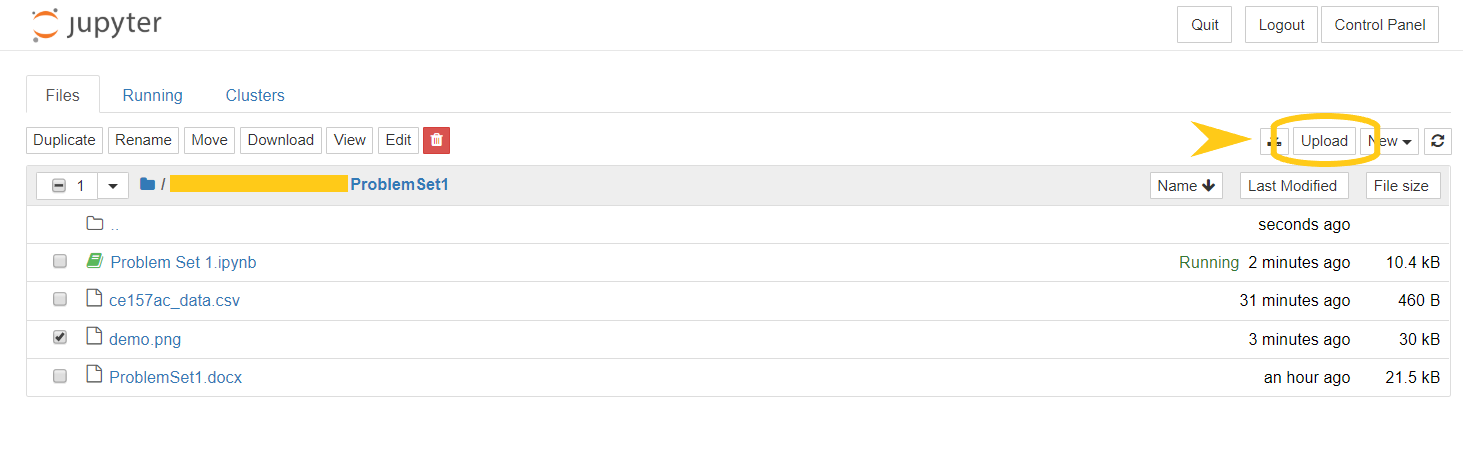
\includegraphics{images/demo.png} Once both images have been uploaded,
you can display them below by replacing the "..." with the
filenames.png. Make sure to give it an appropriate and descriptive
title.

    To display the graph (double click on this cell)

\textbf{Graph Title} \includegraphics{...}

    \begin{Verbatim}[commandchars=\\\{\}]
{\color{incolor}In [{\color{incolor} }]:} \PY{n}{q7\PYZus{}answer} \PY{o}{=} \PY{l+s+sa}{r}\PY{l+s+s2}{\PYZdq{}\PYZdq{}\PYZdq{}}
        
        \PY{l+s+s2}{Put your answer here, replacing this text. Do not take into account the \PYZsh{}\PYZsh{}\PYZsh{} YOUR CODE HERE below}
        
        \PY{l+s+s2}{\PYZdq{}\PYZdq{}\PYZdq{}}
        
        \PY{c+c1}{\PYZsh{} YOUR CODE HERE}
        \PY{k}{raise} \PY{n+ne}{NotImplementedError}\PY{p}{(}\PY{p}{)}
        
        \PY{k}{print}\PY{p}{(}\PY{n}{q7\PYZus{}answer}\PY{p}{)}
\end{Verbatim}


    \begin{Verbatim}[commandchars=\\\{\}]
{\color{incolor}In [{\color{incolor} }]:} \PY{c+c1}{\PYZsh{}Autograder}
        
        \PY{c+c1}{\PYZsh{}\PYZsh{} Autograder?(image has been added and has title)}
\end{Verbatim}


    \subsubsection{Question 8(a)}\label{question-8a}

Reflect on your findings.

Do you think per-capita or total national emissions are the more
appropriate way to do carbon accounting, and why?

    \begin{Verbatim}[commandchars=\\\{\}]
{\color{incolor}In [{\color{incolor} }]:} \PY{n}{q8a\PYZus{}answer} \PY{o}{=} \PY{l+s+sa}{r}\PY{l+s+s2}{\PYZdq{}\PYZdq{}\PYZdq{}}
        
        \PY{l+s+s2}{Put your answer here, replacing this text. Do not take into account the \PYZsh{}\PYZsh{}\PYZsh{} YOUR CODE HERE below}
        
        \PY{l+s+s2}{\PYZdq{}\PYZdq{}\PYZdq{}}
        
        \PY{c+c1}{\PYZsh{} YOUR CODE HERE}
        \PY{k}{raise} \PY{n+ne}{NotImplementedError}\PY{p}{(}\PY{p}{)}
        
        \PY{k}{print}\PY{p}{(}\PY{n}{q8a\PYZus{}answer}\PY{p}{)}
\end{Verbatim}


    \subsubsection{Question 8(b)}\label{question-8b}

Do you think accounting should be based on what a country emits within
its boundaries, or what a country consumes, including emissions from the
production of goods elsewhere?

    \begin{Verbatim}[commandchars=\\\{\}]
{\color{incolor}In [{\color{incolor} }]:} \PY{n}{q8b\PYZus{}answer} \PY{o}{=} \PY{l+s+sa}{r}\PY{l+s+s2}{\PYZdq{}\PYZdq{}\PYZdq{}}
        
        \PY{l+s+s2}{Put your answer here, replacing this text. Do not take into account the \PYZsh{}\PYZsh{}\PYZsh{} YOUR CODE HERE below}
        
        \PY{l+s+s2}{\PYZdq{}\PYZdq{}\PYZdq{}}
        
        \PY{c+c1}{\PYZsh{} YOUR CODE HERE}
        \PY{k}{raise} \PY{n+ne}{NotImplementedError}\PY{p}{(}\PY{p}{)}
        
        \PY{k}{print}\PY{p}{(}\PY{l+m+mi}{8}\PY{n}{b\PYZus{}answer}\PY{p}{)}
\end{Verbatim}


    \subsubsection{Question 8(c)}\label{question-8c}

Do you think countries should reduce their emissions in proportion to

\begin{enumerate}
\def\labelenumi{\alph{enumi})}
\item
  their past emissions
\item
  their level of development \& capacity to reduce
\item
  the degree to which they will be impacted by climate change
\item
  a combination of these, or something else (explain)
\end{enumerate}

    \begin{Verbatim}[commandchars=\\\{\}]
{\color{incolor}In [{\color{incolor} }]:} \PY{n}{q8c\PYZus{}answer} \PY{o}{=} \PY{l+s+sa}{r}\PY{l+s+s2}{\PYZdq{}\PYZdq{}\PYZdq{}}
        
        \PY{l+s+s2}{Put your answer here, replacing this text. Do not take into account the \PYZsh{}\PYZsh{}\PYZsh{} YOUR CODE HERE below}
        
        \PY{l+s+s2}{\PYZdq{}\PYZdq{}\PYZdq{}}
        
        \PY{c+c1}{\PYZsh{} YOUR CODE HERE}
        \PY{k}{raise} \PY{n+ne}{NotImplementedError}\PY{p}{(}\PY{p}{)}
        
        \PY{k}{print}\PY{p}{(}\PY{n}{q8c\PYZus{}answer}\PY{p}{)}
\end{Verbatim}


    \subsection{Final Survey }\label{final-survey}

Congrats! You've finished the final Jupyter Notebook assignment! The
Division of Data Sciences and Information would like to ask you to
please fill this survey out as a part of your assignment. We would like
to improve the module for future semesters, and would really appreciate
it if you took the time to fill this out so we can better serve you!

Please make sure you are logged into your Berkeley (.edu) email address
to access the form. \#\#\#
\href{https://goo.gl/forms/FqSRIYCzAAOfZ5Bv2}{Survey Link}

Alternatively, please copy and paste this link into your URL bar:
https://goo.gl/forms/FqSRIYCzAAOfZ5Bv2

    \subsection{Saving the Notebook as an
HTML}\label{saving-the-notebook-as-an-html}

Congrats on finishing your final notebook! As usual, you will be
submitting this notebook as an HTML file. To turn in this lab assignment
follow the steps below:

\begin{enumerate}
\def\labelenumi{\arabic{enumi}.}
\tightlist
\item
  In the toolbar above, click on File → Download as → HTML
\item
  The file should have been saved in an HTML format in your downloads
  folder.
\item
  Click to open in a web browser of your choice to make sure that
  everything looks okay.
\end{enumerate}


    % Add a bibliography block to the postdoc
    
    
    
    \end{document}
